\begin{center}
    \begin{figure}[H]
        \centering

        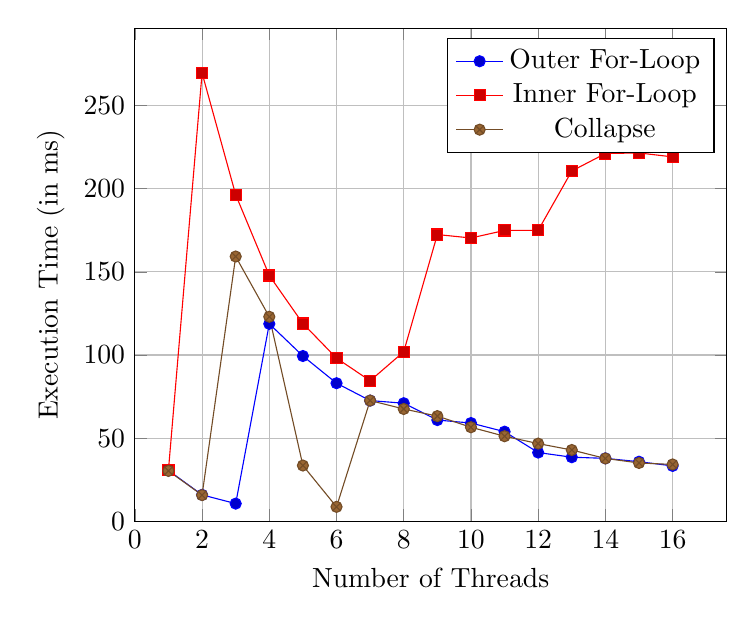
\begin{tikzpicture}
            \begin{axis}[
                title={},
                width=0.75\textwidth,
                xlabel={Number of Threads},
                ylabel={Execution Time (in ms)},
                xmin=0,
                ymin=0,
                grid=major
            ]
                \addplot coordinates {
                    (1,30.5744)(2,15.9054)(3,10.6403)(4,118.764)(5,99.3969)(6,83.0441)(7,72.5946)(8,71.0114)(9,60.8864)(10,59.0989)(11,53.8984)(12,41.3449)(13,38.5431)(14,37.859)(15,35.84)(16,33.3233)
                };
                \addlegendentry{Outer For-Loop}

                \addplot coordinates {
                    (1,30.9466)(2,269.554)(3,196.369)(4,147.807)(5,118.939)(6,98.1236)(7,84.5119)(8,101.967)(9,172.437)(10,170.371)(11,174.918)(12,174.982)(13,210.657)(14,221.162)(15,221.516)(16,219.138)
                };
                \addlegendentry{Inner For-Loop}       

                \addplot coordinates {
                    (1,30.3246)(2,15.7525)(3,159.229)(4,123.008)(5,33.5471)(6,8.6973)(7,72.6206)(8,67.5459)(9,63.2531)(10,56.5625)(11,51.1589)(12,46.733)(13,42.8813)(14,37.8017)(15,35.0829)(16,34.1962)
                };
                \addlegendentry{Collapse}
            \end{axis}
        \end{tikzpicture}
        \caption{HSV Performance Tests dice.png}
    \end{figure}
\end{center}